\documentclass[aspectratio=169]{beamer}


\usepackage[utf8]{inputenc}
\usepackage{amsmath}
\usepackage{amsfonts}
\usepackage{amssymb}
\usepackage{graphicx}
\usepackage{ragged2e}  % `\justifying` text
\usepackage{booktabs}  % Tables
\usepackage{tabularx}
\usepackage{tikz}      % Diagrams
\usetikzlibrary{calc, shapes, backgrounds}
\usepackage{amsmath}
\usepackage{amssymb}
\usepackage{dsfont}
\usepackage{url}       % `\url
\usepackage{listings}  % Code listings
\usepackage[T1]{fontenc}
\usepackage{subcaption}

\usepackage{eurosym}
\usepackage{polyglossia}
\setdefaultlanguage{english}
\usepackage[autostyle,german=guillemets]{csquotes}
\usepackage[linesnumbered,ruled,vlined]{algorithm2e}

\usepackage{xcolor}
\usepackage{listings}
\usepackage{caption}


\usepackage{xcolor}
\usepackage{listings}
\usepackage{caption}
\DeclareCaptionFont{white}{\color{white}}
\DeclareCaptionFormat{listing}{%
	\parbox{\textwidth}{\colorbox{gray}{\parbox{\textwidth}{#1#2#3}}\vskip-4pt}}
\captionsetup[lstlisting]{format=listing,labelfont=white,textfont=white}
\lstset{frame=lrb,xleftmargin=\fboxsep,xrightmargin=-\fboxsep}

\lstset{
	% numbers=left,
	breaklines=true,
	% backgroundcolor=\color{light-gray},
	tabsize=4,
	% basicstyle=\ttfamily,
	literate={\ \ }{{\ }}1	
}


\newenvironment{figure*}%
{\begin{figure}}
	{\end{figure}}


\usepackage{theme/beamerthemehbrs}

\title{Compliant Manipulation using Reinforcement Learning guided by Task Specification}
\subtitle{Master Thesis}
\author{Abhishek Padalkar}
\institute[HBRS]{Hochschule Bonn-Rhein-Sieg}
\date{\today}
\subject{Test beamer}

% \thirdpartylogo{path/to/your/image}


\begin{document}
{
\begin{frame}
\titlepage
\end{frame}
}

\begin{frame}{Motivation}
	\begin{itemize}
		\item Compliant manipulation is a must to have ability for collaborative and service robots.
		\item Robots need to deal with:
		\begin{itemize}
			\item Inaccuracy in the geometric model of the world
			\item Contact forces
			\item External forces due to collision and other agents
		\end{itemize}
		
		
		\item Limitations of model-based approaches:
		\begin{itemize}
			\item Lack of precise model of contact forces
			\item High computational complexity 	
		\end{itemize} 
		
		\item Limitations of learning based solutions:
		\begin{itemize}
			\item Reinforcement learning requires high number of interactions.
			
			\item Accuracy of simulation affects the learned behavior and transferability of solution.
				
		\end{itemize}
		\end{itemize}
\end{frame}

\begin{frame}
	\begin{minipage}[t]{0.49\textwidth}
	\begin{figure}
		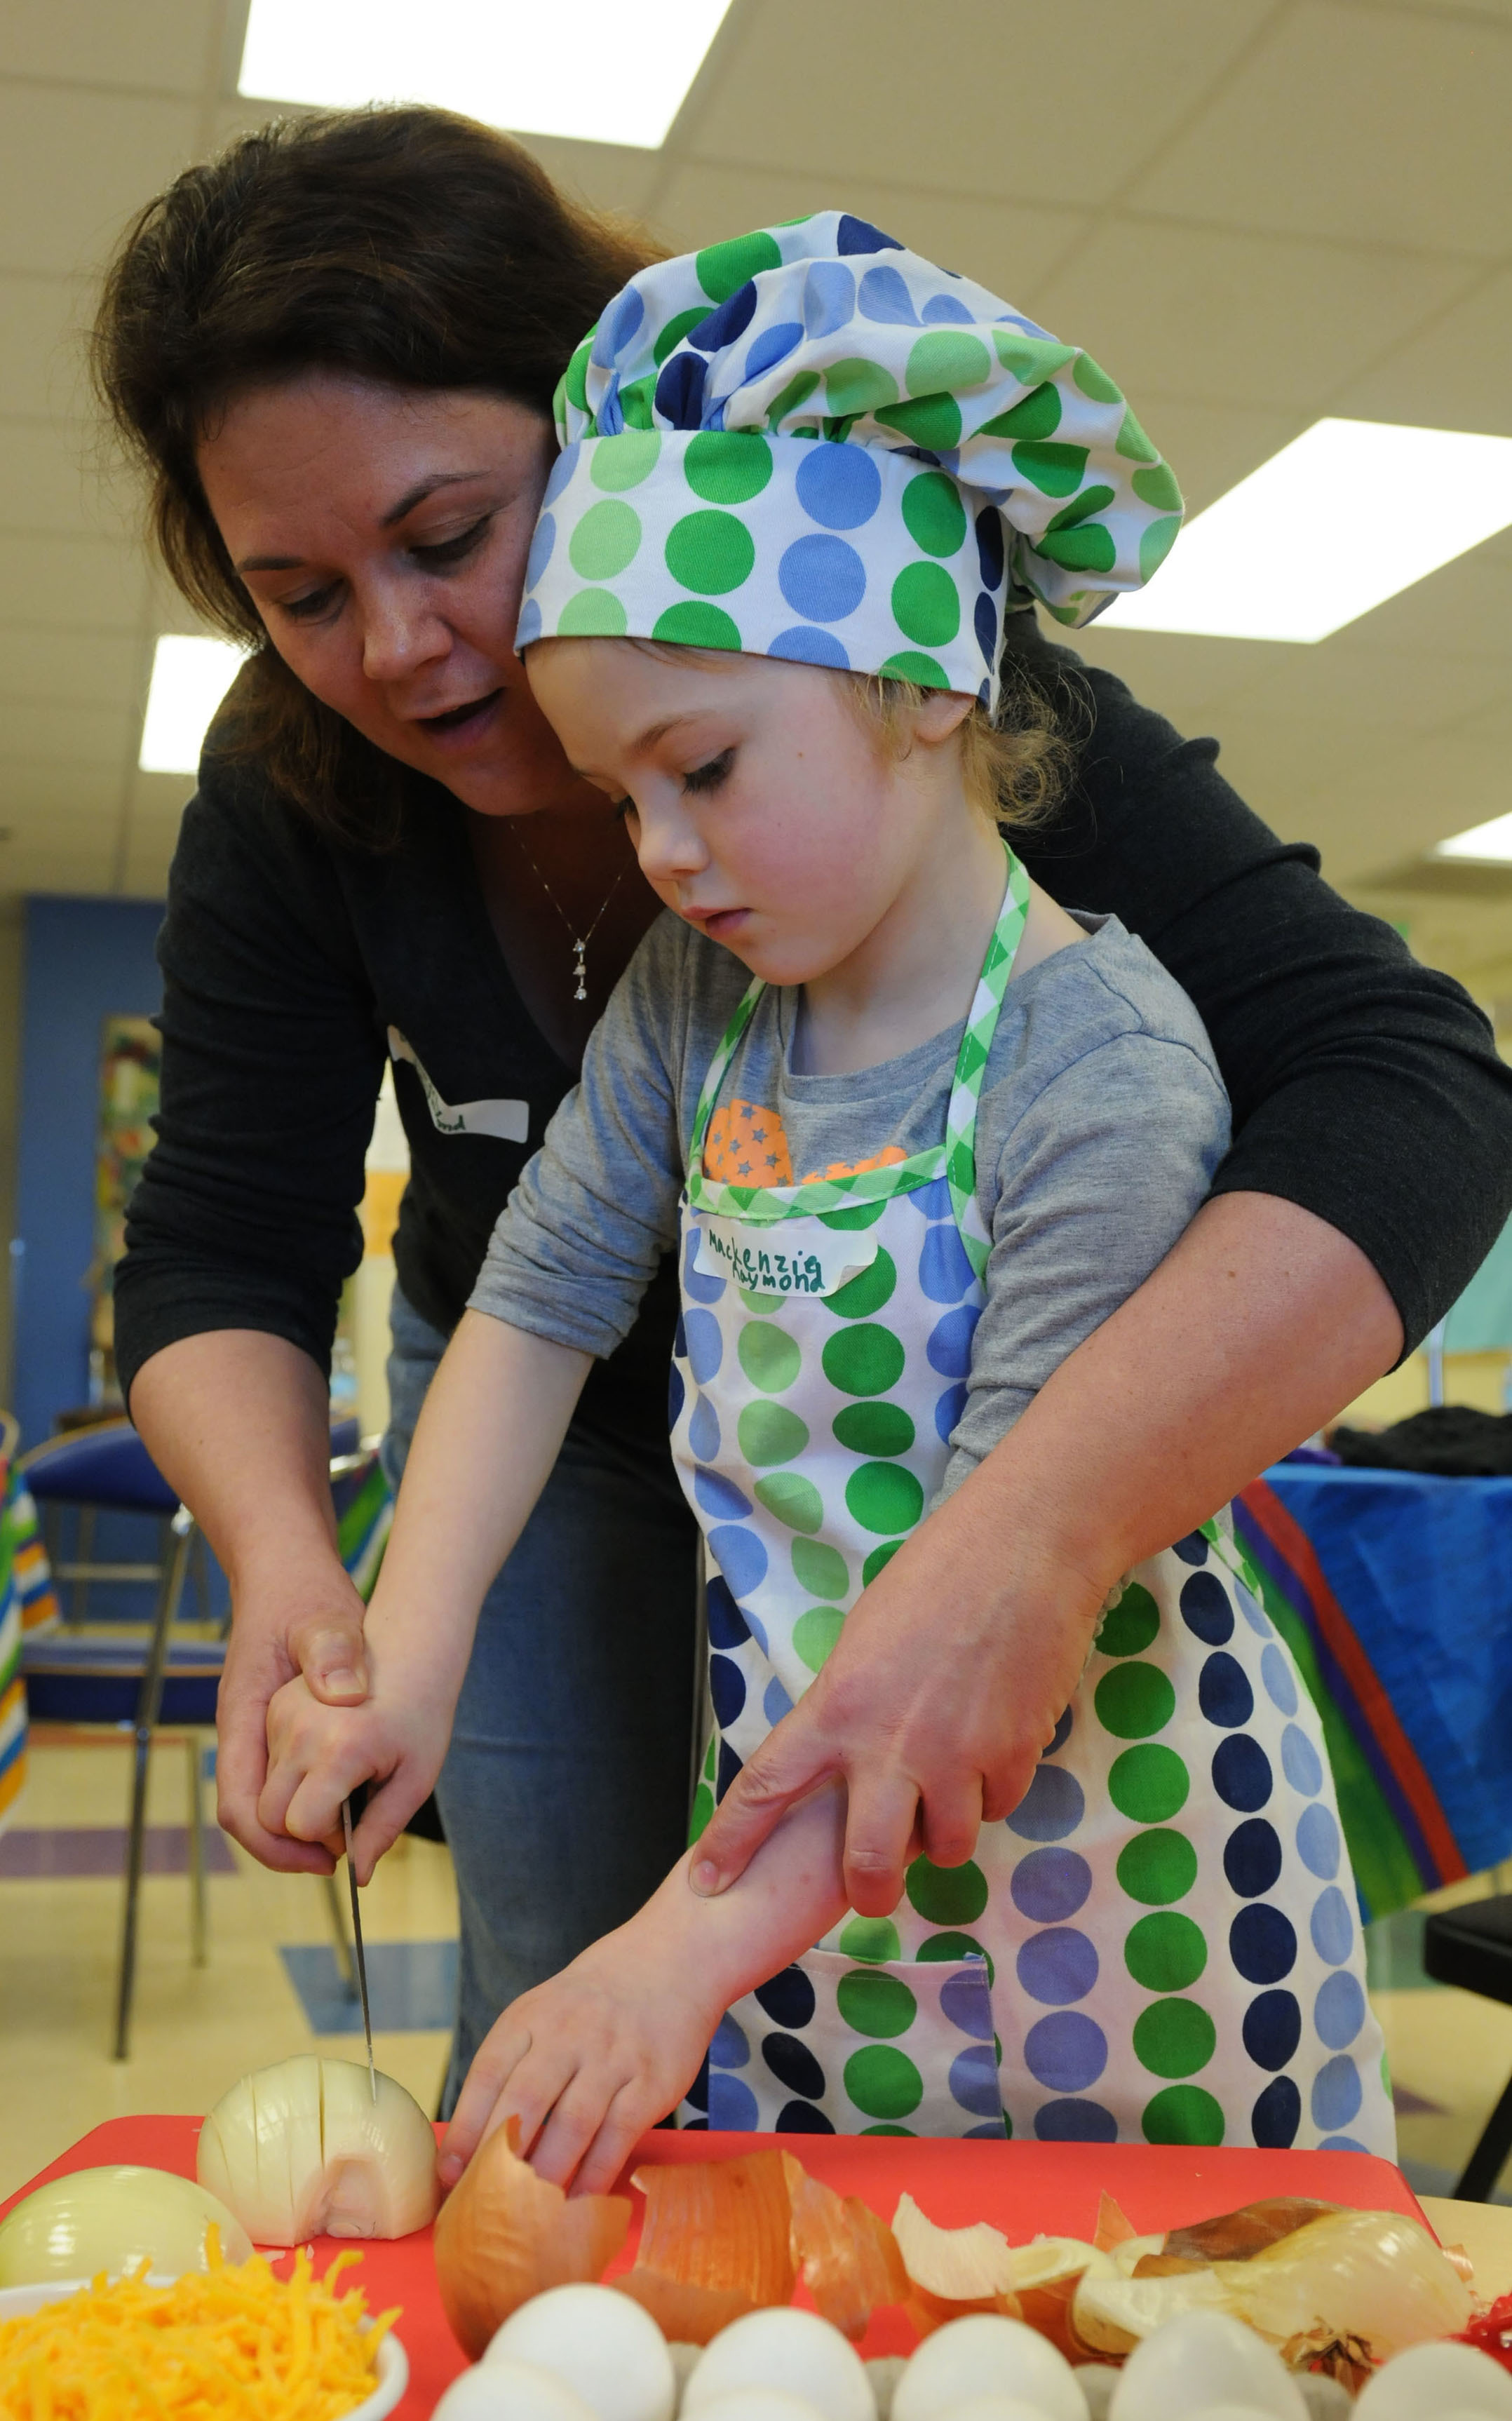
\includegraphics[width=0.6\textwidth]{images/mother_child}
		\caption{Mother teaching child to cut vegetables.}
	\end{figure}
		\end{minipage}
		\hfil
	\begin{minipage}[t]{0.49\textwidth}
			\begin{itemize}
				\item Humans learn multiple tasks through demonstrations and descriptions.
				\item Vital knowledge about motion is extracted and utilized.
				\item The task is then perfected with experience.
				\item Similarly, a task can be described or specified to a robot. 
			\end{itemize}
		\end{minipage}
		
\end{frame}

\begin{frame}{Problem Statement}
	Develop a learning based approach for achieving compliant manipulation that allows to exploit partial/incomplete models of the task and the environment provided by the task specification.
	\vspace{0.5cm}
	
	Two sub-problems:
	\begin{itemize}
		\item Model the easy-to-model knowledge about tasks using task specification framework.
		
		\item Use Reinforcement Learning for learning gradually more complete and robust action models for compliant manipulation tasks.
	\end{itemize}
	
	
	We demonstrate our approach on two demo tasks:
	\begin{itemize}
		\item Opening door, and
		\item Cutting vegetables.
	\end{itemize}
\end{frame}

\begin{frame}[fragile]{Related Work}{\small Task Specification Methods}
	\vspace{-0.5cm}
	\begin{itemize}
		\item Industrial task specification languages like KUKA Robot Language 
		\begin{itemize}
			\item Reliable
			\item Difficult to integrate sensory feedbacks
			\item Limited expressive power \cite{leidner2017cognitive}
	\end{itemize}
		\item Task Frame Formalism specifies the task in \textit{task frame} or \textit{compliance frame}, by defining motion or force in each DoF\cite{nagele2018prototype, mason1981compliance}. 
	\end{itemize}

	\begin{itemize}
		\item Leidner presents symbolic representation of the task in PDDL along with the geometric representation of the task using sequence of low level movement sequences. 
		\item iTaSC synthesizes control inputs by solving an optimization problem considering the task space constraints \cite{DeSchutter-ijrr2007, DecreBruyninckxDeSchutter2013, decre09}. 
		
	\end{itemize}
\end{frame}

\begin{frame}[allowframebreaks]{~}{Reinforcement Learning}
	\vspace{-0.5cm}
	\begin{itemize}
		\item {Model-based} reinforcement learning learns the model of environment as well as policy for performing the task.
		\item Number of interactions required can be very high for learning model of the environment.
		\item {Model-free} reinforcement learning learns value functions without learning the model of the environment. 
		\item Policy search methods are model-free learning methods which directly learn policy to take action in current observable state without learning value function.
		\framebreak
		\item Policy search methods are used heavily in robot control due to their ability to handle high dimensional state-action space.
		\item Algorithms:
		\begin{itemize}
			
			\item Finite difference method : Learns by comparing returns with baseline after exploration in parameter space.
			\item Likelihood ratio method / REINFORCE : Uses policy gradient theorem  
			\item Natural actor critic algorithm 
			\item Path integral policy improvement (PI$^{2}$)
			\item Expectation-maximization method (PoWER) : Learns by exploration in the parameter space and by weighing the exploration by returns
		\end{itemize} 
		
	\end{itemize}
\end{frame}

\begin{frame}
		\vspace{-0.5cm}
	Door opening task
	\begin{itemize}
		\item Motion synthesis using the geometric model of the door : requires accurate model of door
		\item Adaptive control along with on-line estimation of the door parameters using force-torque sensors : sensor noise affects the parameter estimation
		\item Learning force policies using reinforcement learning : requires numerous interactions with environment
		\item Learning the task from human demonstrations using Dynamic Motion Primitives : not generalizable for different doors
	\end{itemize}
	
	\textbf{Vegetable cutting task}
	\begin{itemize}
		\item Deep recurrent neural network with model predictive control : requires large amount of data to learn the model 
		\item Using sequence of Dynamic Motion Primitives : purely motion-based approach
	\end{itemize}
\end{frame}

\begin{frame}{Solution}
	\begin{itemize}
		
		\item Provide task specification using Task Frame Formalism (TFF), which also contains a policy to be learned by reinforcement leaning for generating control commands.
		
		\item Design policy for control command generation in the task specification. This policy can be a engineered policy for a well understood problem or can be a generic parameterized policy e.g. neural network or radial basis function network.
		
		\item Design a reward function for the given task.
		
		\item Use existing reinforcement learning methods to learn parameters of the policy to maximize given reward function by carrying out trials in the environment.
	\end{itemize}
\end{frame}
\begin{frame}
		\vspace{-0.5cm}\hspace{0.5cm}
	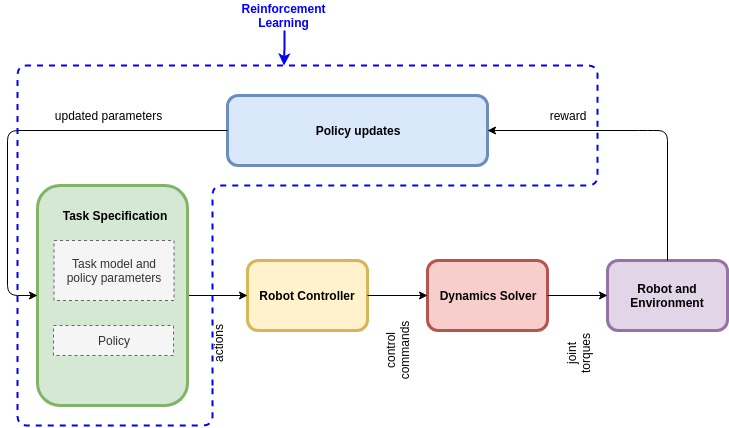
\includegraphics[width=0.9\textwidth]{images/composition}
\end{frame}

\begin{frame}{Task Specification using Task frame formalism}
		\vspace{-0.3cm}
		
	Task frame formalism provides guidelines for identifying \alert{reciprocal degrees of freedom} and task specification using them.
	
	\hspace{0.5cm} The frame is chosen such that the motion does not generate power against reaction forces.
		
	%\newgeometry{textwidth=11.53cm}
	%\vskip1ex
	\begin{minipage}[b]{0.49\textwidth}
		
		\begin{figure}
			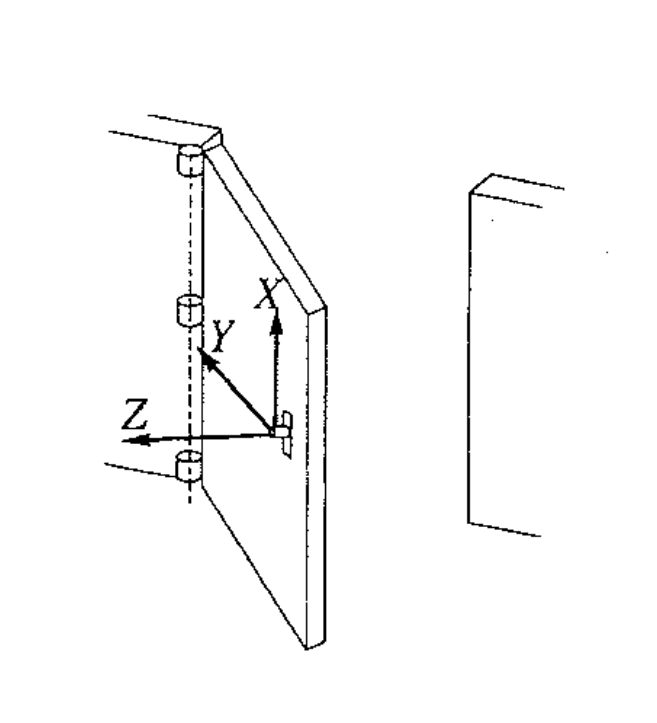
\includegraphics[width=0.6\textwidth]{images/tff_open_doora.png}
			\caption{\scriptsize Task frame selection for door opening task \\ ~}
		\end{figure}
	\end{minipage}
	\hfill
	\begin{minipage}[b]{0.49\textwidth}
		\begin{figure}

			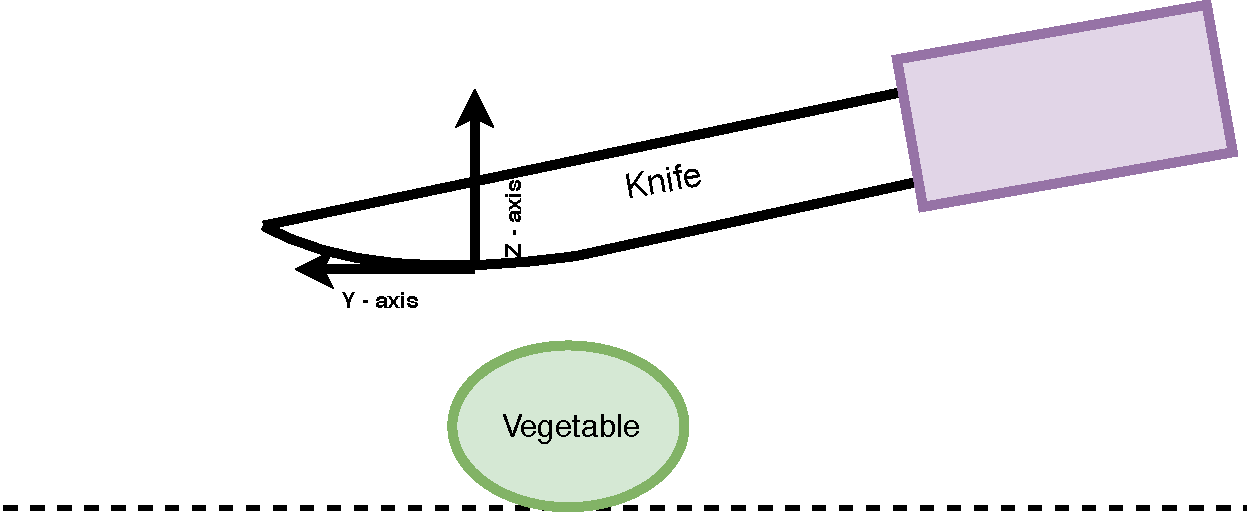
\includegraphics[width=0.8\textwidth]{images/tff_knife}
			\caption{\scriptsize Task frame selection for vegetable cutting task}
						%\vspace{1cm}
		\end{figure}
	\end{minipage}
\end{frame}

\begin{frame}[fragile]{~}{Task specification for opening door:}
	\begin{figure}
		\begin{lstlisting}[label=tff-open-door-a,caption=Task Specification using TFF: Open Door]
        move compliantly {
        with task frame directions
        xt: force 0 N
        yt: force 0 N
        zt: velocity v m/sec
        axt: force 0 Nm
        ayt: force 0 Nm
        azt: force 0 Nm
    }until chord length > d m or force z > f N \end{lstlisting}
	\end{figure}
\end{frame}

\begin{frame}[fragile]{~}{Task specification for cutting vegetables:}
	\begin{figure}
		\begin{lstlisting}[label=cut_vegies,caption=Cut vegetables]
        move compliantly {
        with task frame directions
        xt: velocity 0 m/s 
        yt: velocity v(t) m/s
        zt: force f(environment, robot, task) N
        axt: velocity 0 rad/s
        ayt: velocity 0 rad/s
        azt: velocity 0 rad/s
    }until distance y > d m \end{lstlisting}
	\end{figure}
\end{frame}

\begin{frame}{Reinforcement Learning Algorithms}{REINFORCE}
	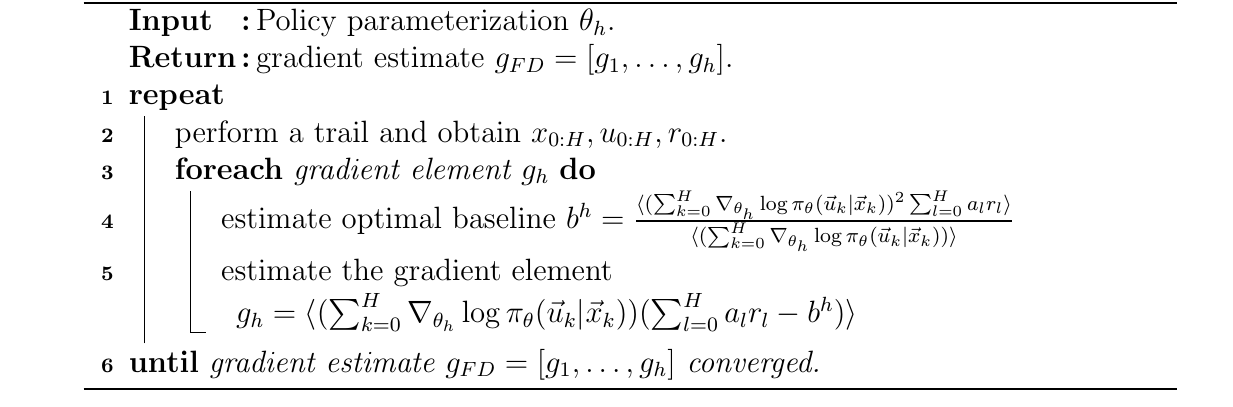
\includegraphics[width=\textwidth]{images/reinforce}
	
	\begin{itemize}
		\small
		\item Uses policy gradient theorem to estimate the gradient of the parameters.
		\item Adds exploration noise in the actions at every discrete time step.
	\end{itemize}
\end{frame}

\begin{frame}{~}{Policy learning by Weighting Exploration with the Returns (PoWER)}
	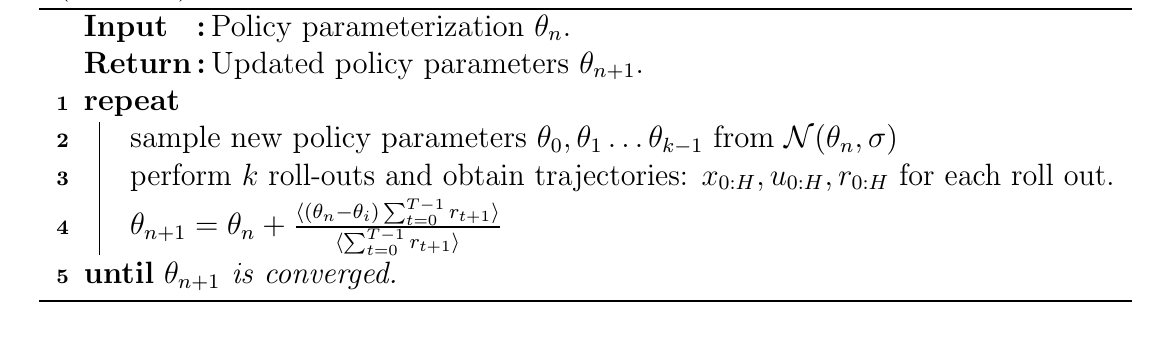
\includegraphics[width=\textwidth]{images/power}
	
	\begin{itemize}
		\small 
		\item Uses expectation-maximization method to estimate the gradient of the parameters.
		\item Adds exploration noise in the parameters at the beginning of the episode.
	\end{itemize}
\end{frame}


\begin{frame}{Policy Representation and Reward Function}
	\vspace{-0.7cm}
	\small
	\begin{itemize}
		\item Linear policy \begin{align}
		f = -(A\dot{y} + B(0.5^{2} - (0.5 - \phi_{y})^{2}) + C(1-\phi_{z}))
		\end{align}
		\item Gaussian policy 
			\vspace{-0.7cm}
		\begin{align}
		f = -(A\dot{y} + B(0.5^{2} - (0.5 - \phi_{y}^{2})) + \sum_{i=0}^{N-1}W\psi_{i}(\phi_{z}))
		\end{align}
					\vspace{-0.7cm}
		\begin{align}
		\psi_{i}(\phi_{z}) = \frac{1}{\sqrt{2\pi\sigma^{2}}}e^{\frac{(c_{i} - \phi_{z})}{2\sigma^{2}}}
		\end{align}
		\vspace{-0.5cm}
			\item Where reward function used is : 
			\begin{align}
			r = C_{1}*\phi_{z}^{2} - C_{2}*f_{z}^{2}
			\end{align}
	\end{itemize}
	\vspace{-0.3cm}
	\scriptsize
	where $A, B, C$, and $W$ (weight vector) are policy parameters, $N$ is number of Gaussian functions, $c_{i}$ is the center of $i^{th}$ Gaussian, $\sigma$ is width of Gaussian functions, $\phi_{y}$ and $\phi_{z}$ are cutting phases in Y 
	and Z direction respectively.
\end{frame}

\begin{frame}{Experimental Results: Door opening task}
	\vspace{-0.5cm}
	Experiments were performed with two robots:
	\begin{itemize}
		\small
		\item Schunk LWA4D equipped with Schunk FTM115 force torque module and Schunk Dexterous Hand 
		\item Toyota Human Service Robot (HSR)
	\end{itemize}
	\vspace{-0.4cm}
	\centering
	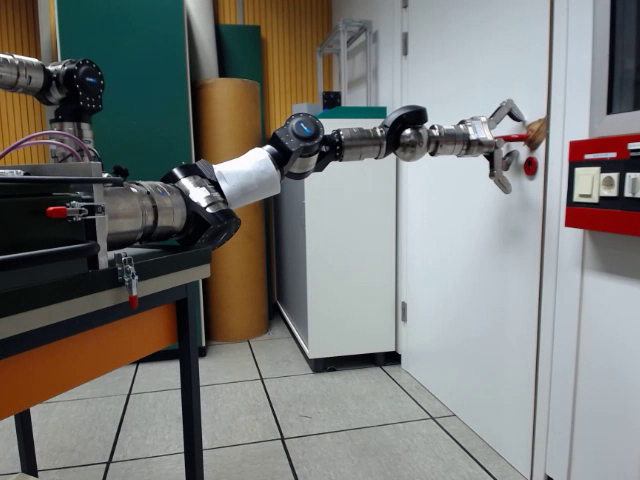
\includegraphics[width=0.45\textwidth]{images/exp/lwa_door}
	\hfil
	\vspace{0.4cm}
	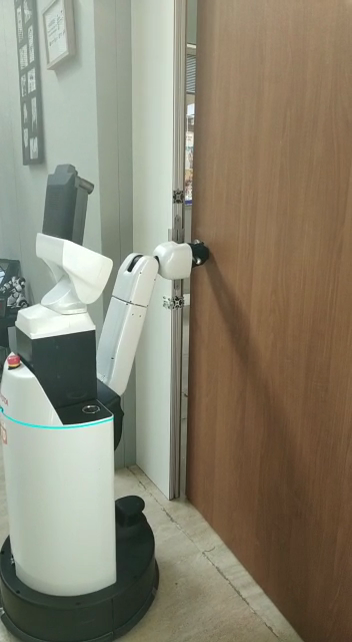
\includegraphics[width=0.2\textwidth]{images/exp/hsr_door} 
\end{frame}

\begin{frame}
	%\vspace{-0.5cm}
	Schunk LWA4D opening unlatched door
	\vspace{-0.5cm}
	\begin{figure}[h]
		\centering
		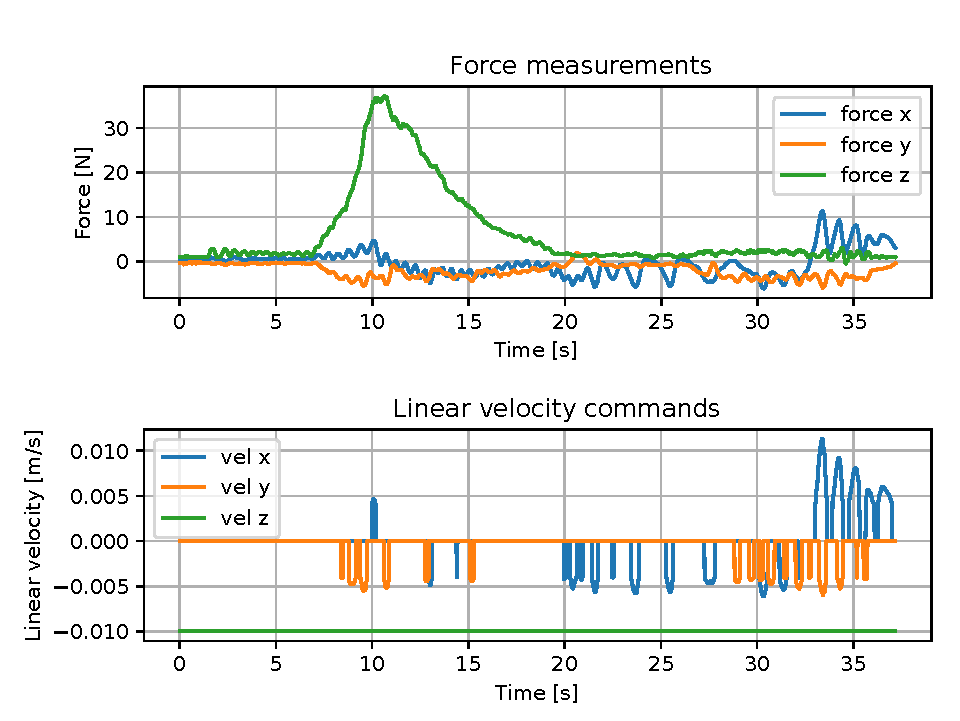
\includegraphics[width=0.7\textwidth]{images/exp/f-vn.pdf}
			\vspace{-0.3cm}
		\caption{Force readings at TCP and linear velocity applied to TCP}
		\label{EX:f-v}
	\end{figure}
\end{frame}


\begin{frame}
	Schunk LWA4D opening unlatched door
	\vspace{-0.4cm}
	\begin{figure}[t]
		\centering
		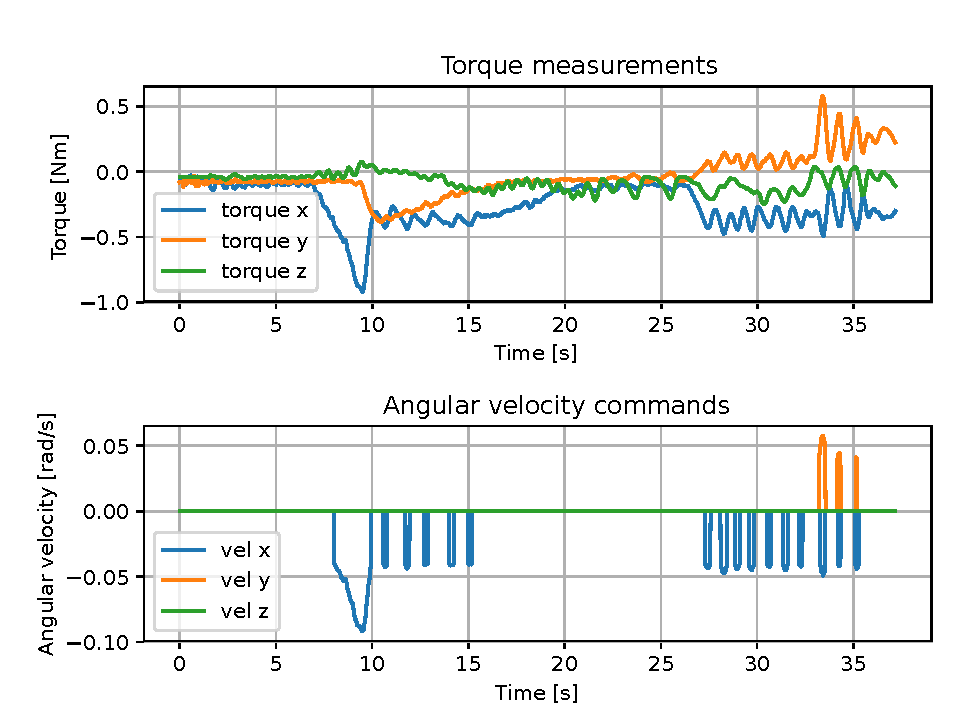
\includegraphics[width=0.7\textwidth]{images/exp/t-wn.pdf}
		\vspace{-0.3cm}
		\caption{Torque readings at TCP and velocity angular velocity applied at TCP}
		\label{EX:t-w}
	\end{figure}
\end{frame}

\begin{frame}
	Schunk LWA4D opening unlatched door
	\vspace{-0.3cm}
	\begin{figure}[t]
		\centering
		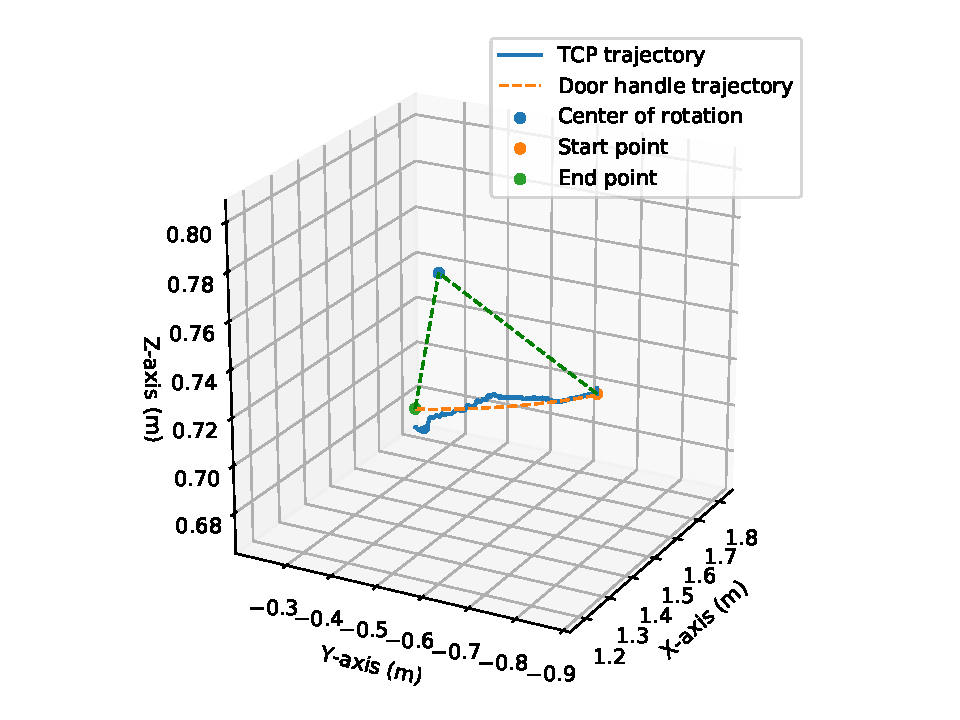
\includegraphics[width=0.7\textwidth]{images/exp/traj.pdf}
			\vspace{-0.3cm}
		\caption{Geometric analysis of trajectory traced by TCP}
		\label{EX:traj}
	\end{figure}
\end{frame}

\begin{frame}
	Toyota HSR trying to open jammed door
	\vspace{-0.4cm}
	\begin{figure}[h]
		\centering
		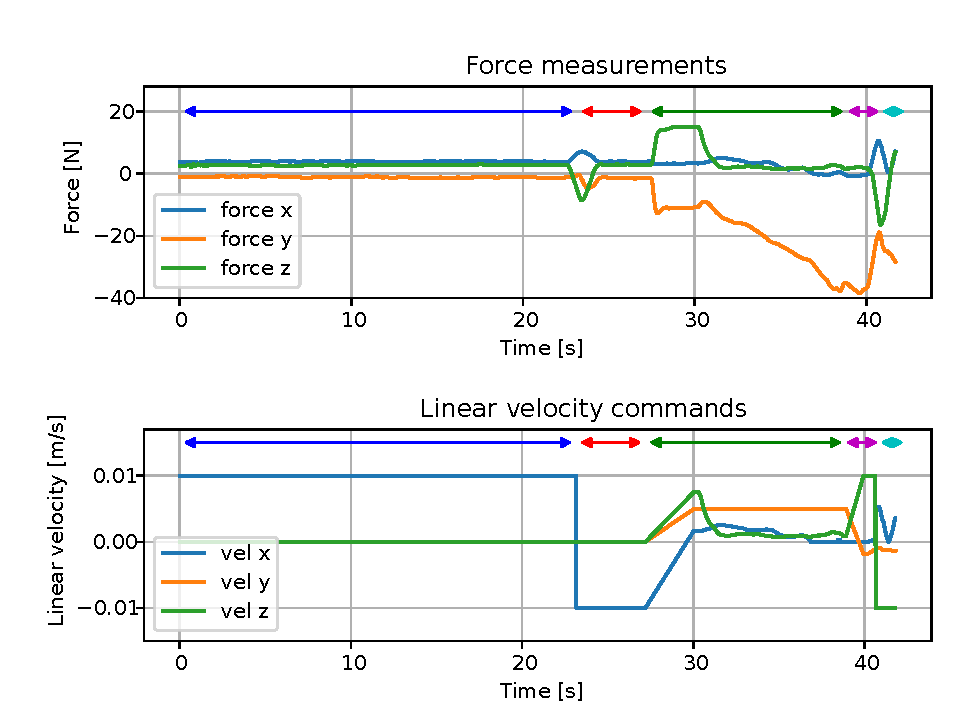
\includegraphics[width=0.7\textwidth]{images/exp/8776_fn.pdf}
		\vspace{-0.3cm}
		\caption{Force readings at TCP and linear velocity applied to TCP}
	\end{figure}
\end{frame}


\begin{frame}
	Toyota HSR trying to open jammed door
	\vspace{-0.4cm}
	\begin{figure}[t]
		\centering
		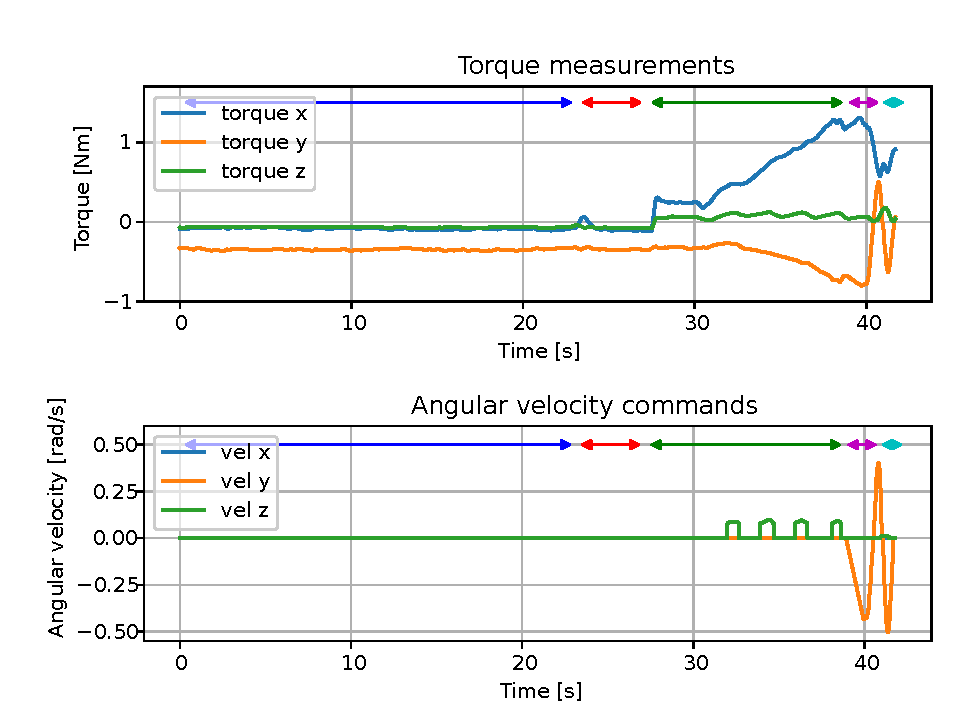
\includegraphics[width=0.7\textwidth]{images/exp/8776n.pdf}
			\vspace{-0.3cm}
		\caption{Torque readings at TCP and velocity angular velocity applied at TCP}
		
	\end{figure}
\end{frame}

\begin{frame}
	Toyota HSR trying to open jammed door
	\vspace{-0.3cm}
	\begin{figure}[t]
		\centering
		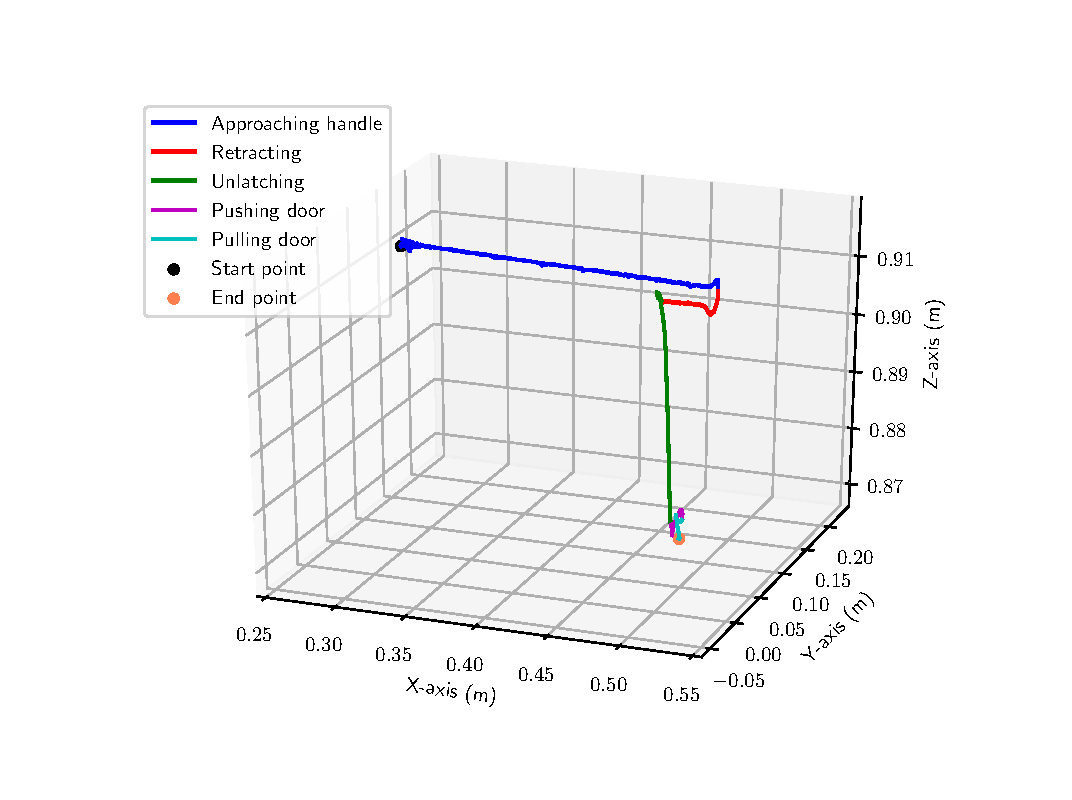
\includegraphics[width=0.7\textwidth]{images/exp/8776_traj.pdf}
			\vspace{-0.3cm}
		\caption{Geometric analysis of trajectory traced by TCP}
		
	\end{figure}
\end{frame}


\begin{frame}{~}{Discussion}
	\begin{itemize}
		
		\item Schunk LWA4D was able to open the door every time in 27 trials.
		\item Robot was able to open the door in the presence of a bump on the floor.
		\item Toyota HSR robot was successful in detecting the opening direction of door and in determining whether the door is jammed or not.
		
		\item The chord length traced while opening door varies because :
		\begin{itemize}
			\item One or more joint limits reached
			\item Operation was stopped to avoid self-collision
		\end{itemize}
		\item Oscillations were observed in the trajectory because of :
		\begin{itemize}
			\item Drift in the sensor readings over time
			\item Delay in motion command update
		\end{itemize}
		
	\end{itemize}
\end{frame}


\begin{frame}{Vegetable Cutting Experiment}
		\vspace{-0.5cm}
		Testing algorithm in simulation

		\begin{minipage}[t]{0.51\textwidth}
		\begin{figure}
			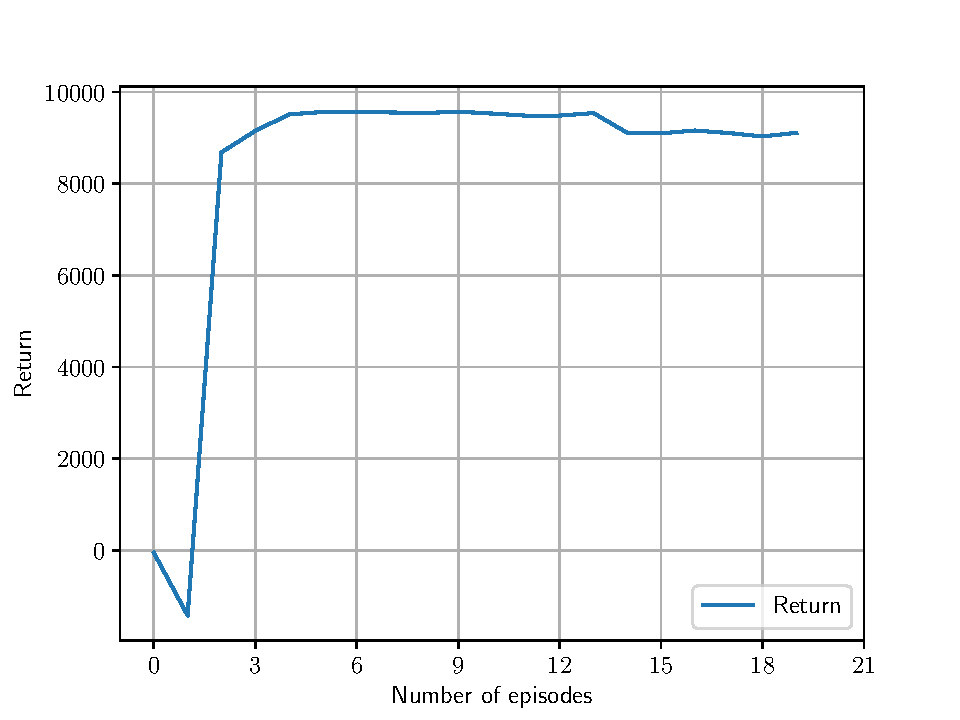
\includegraphics[width=\textwidth]{images/exp/cut/sim_return}
			\caption{Performance of REINFORCE algorithm in simulation}
		\end{figure}
		\end{minipage}
		\hfill
		\begin{minipage}[t]{0.47\textwidth}
			\small
			\vspace{0.5cm}
				\begin{itemize}
					\item Vegetable cutting task was simulated as motion of object through a viscous medium.
					\item REINFORCE algorithm successfully learned cutting policy.
				\end{itemize}
		\end{minipage}
\end{frame}

\begin{frame}
	Experiments with KUKA LWR 4+
	\begin{figure}
		\centering
		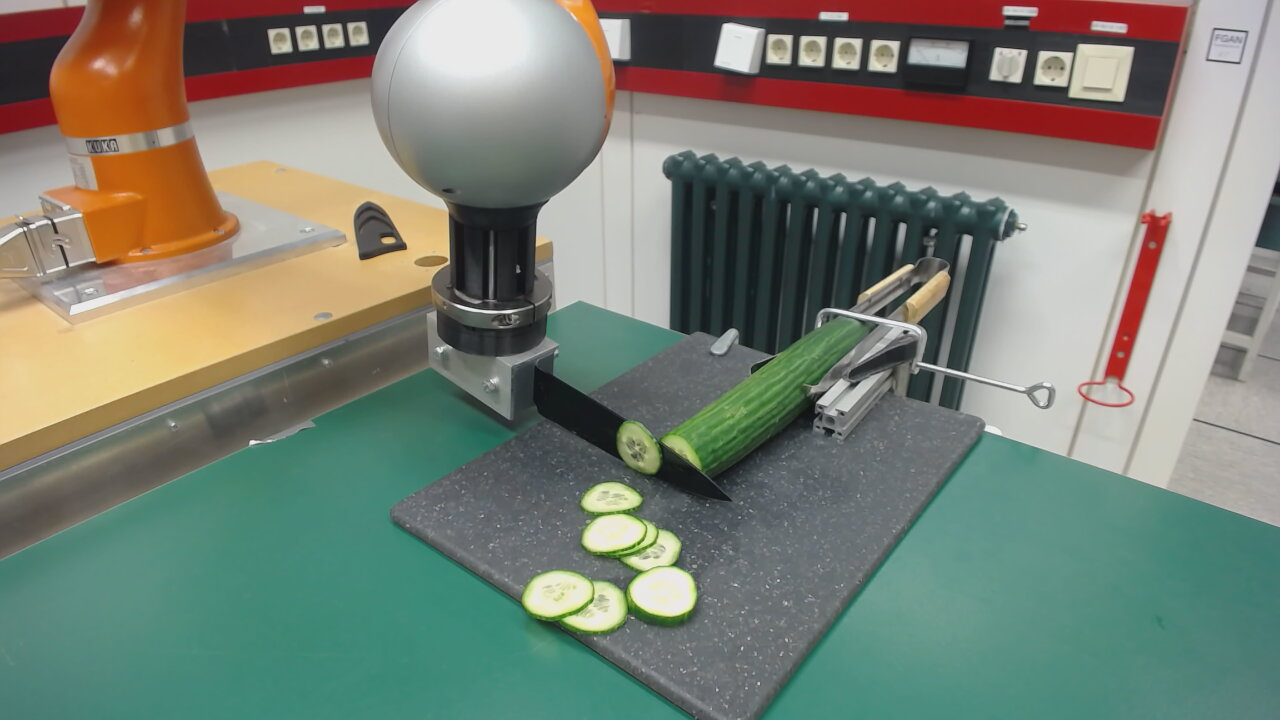
\includegraphics[width=0.8\textwidth]{images/exp/cut_veg_exp}
		\caption{KUKA LWR 4+ cutting vegetable}
	\end{figure}
\end{frame}

\begin{frame}
	Learning Force Policy with REINFOCE Algorithm
	%\vskip1ex
	\begin{minipage}[t]{0.51\textwidth}
		\begin{figure}
			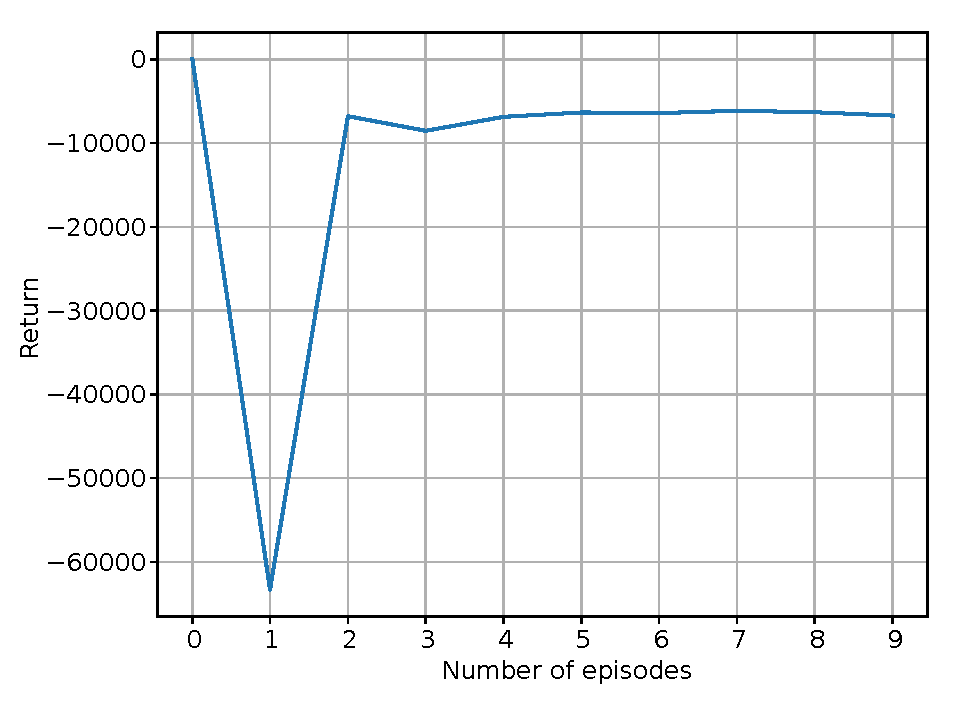
\includegraphics[width=0.95\textwidth]{images/exp/cut/reinf_returnn}
			\caption{\scriptsize Performance of REINFORCE algorithm with KUKA LWR 4+}
		\end{figure}
	\end{minipage}
	\hfill
	\begin{minipage}[t]{0.47\textwidth}
		\vspace{0.5cm}
		REINFORCE algorithm fails to learn force policy:
		\begin{itemize}
			\small
			\item RINFORCE uses high frequency noise for exploration in action space.
			\item The task and robot dynamics acts as a low-pass filter.
			\item Contact dynamics also acts as low pass filter.
			\item Hence noise is damped and REINFORCE does not converge.
		\end{itemize}
	\end{minipage}
\end{frame}


\begin{frame}
	Learning Force Policy with PoWER Algorithm
	%\vskip1ex
	\begin{minipage}[t]{0.51\textwidth}
		\begin{figure}
			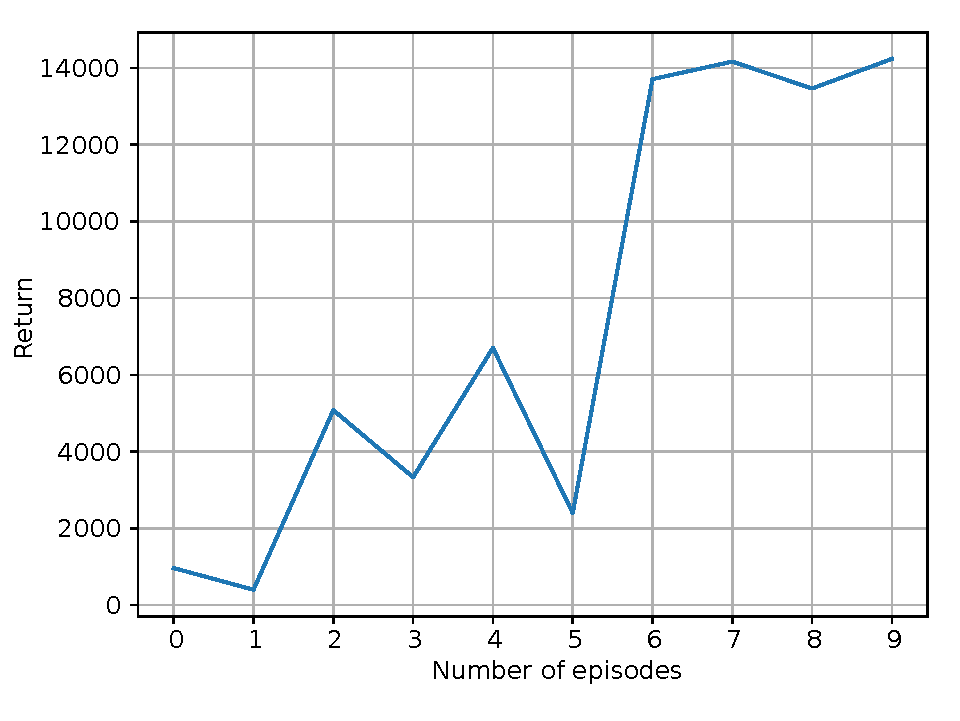
\includegraphics[width=0.95\textwidth]{images/exp/cut/power_return1n}
			\caption{\scriptsize Performance of PoWER algorithm with KUKA LWR 4+ using linear policy}
		\end{figure}
	\end{minipage}
	\hfill
	\begin{minipage}[t]{0.47\textwidth}
		\vspace{0.5cm}
		PoWER algorithm successfully learns force policy:
		\begin{itemize}
			\item Policy was learned after 6 episodes.
			\item Effective exploration was possible because of low frequency noise.
		\end{itemize}
	\end{minipage}
\end{frame}


\begin{frame}
	Cutting cucumber with generated policy
	
	%\vskip1ex
	\begin{minipage}[t]{0.49\textwidth}
		\begin{figure}
			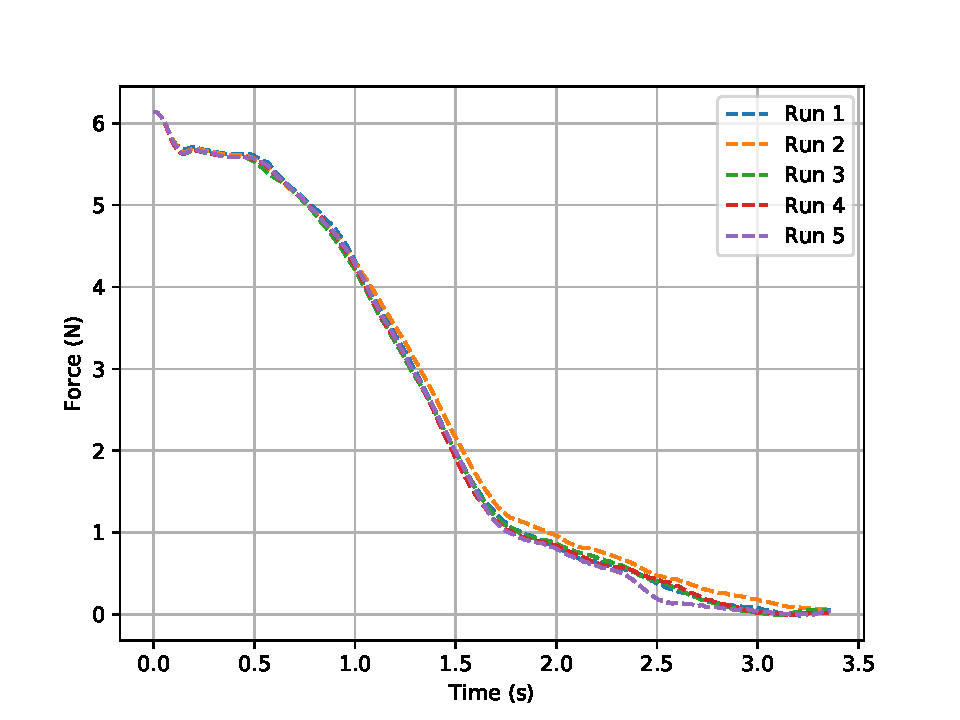
\includegraphics[width=\textwidth]{images/exp/cut/power_f1}
			\caption{\scriptsize Force generated by linear policy while cutting cucumber}
		\end{figure}
	\end{minipage}
	\hfill
	\begin{minipage}[t]{0.49\textwidth}
		
		\begin{figure}
			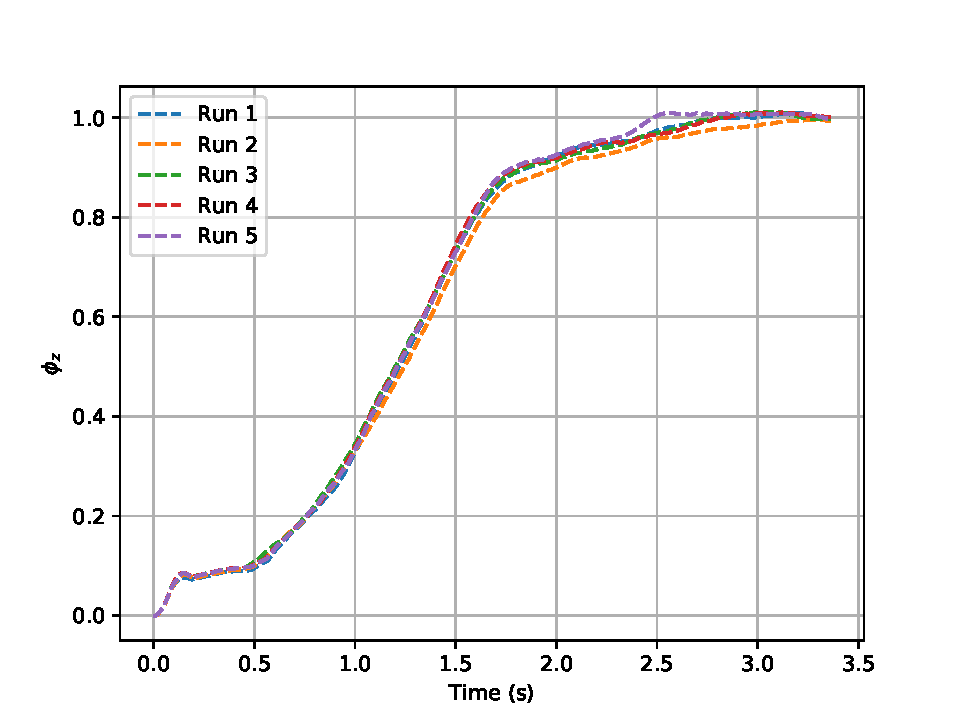
\includegraphics[width=\textwidth]{images/exp/cut/power_ph_z1}
			\caption{\scriptsize Cutting phase $\phi_{z}$ in Z-direction}
		\end{figure}
	\end{minipage}
\end{frame}




\begin{frame}
	Learning Force Policy with PoWER Algorithm
	
	%\vskip1ex
	\begin{minipage}[t]{0.51\textwidth}
		\begin{figure}
			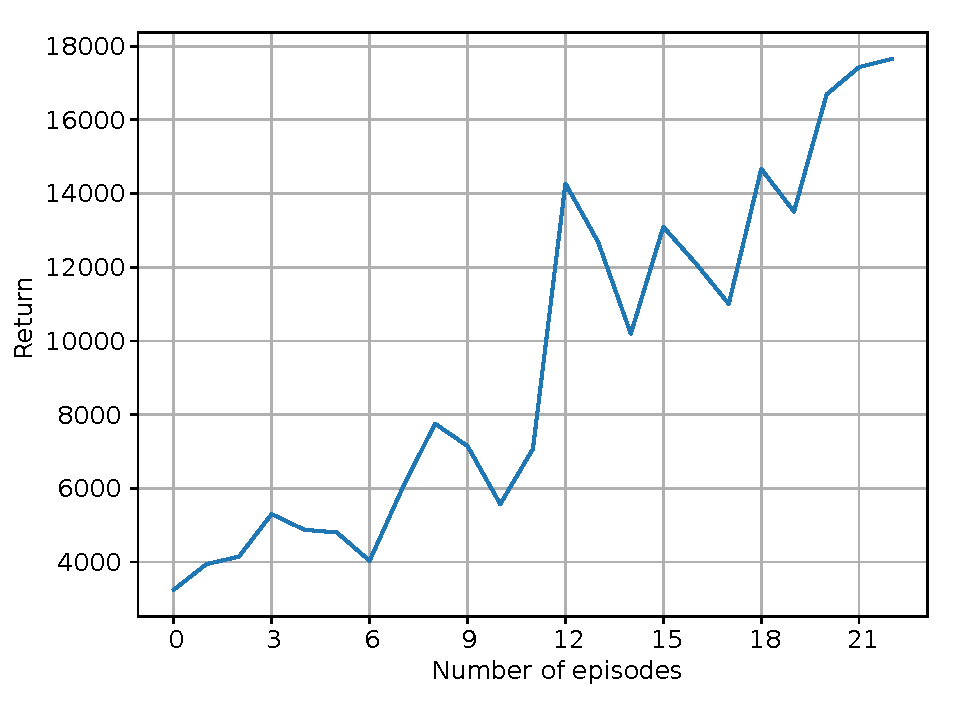
\includegraphics[width=0.95\textwidth]{images/exp/cut/power_return2n}
			\caption{\scriptsize Performance of PoWER algorithm with KUKA LWR 4+ using linear policy}
		\end{figure}
	\end{minipage}
	\hfill
	\begin{minipage}[t]{0.47\textwidth}
		
		\vspace{0.5cm}
		PoWER algorithm successfully learns force policy:
		\begin{itemize}
			\scriptsize 
			\item Policy was learned after 20 episodes
			\item Increase in number parameters requires more trials to learn the policy.
		\end{itemize}
	\end{minipage}
\end{frame}


\begin{frame}
	Learning Force Policy with PoWER Algorithm
	%\vskip1ex
	\begin{minipage}[t]{0.49\textwidth}
		\begin{figure}
			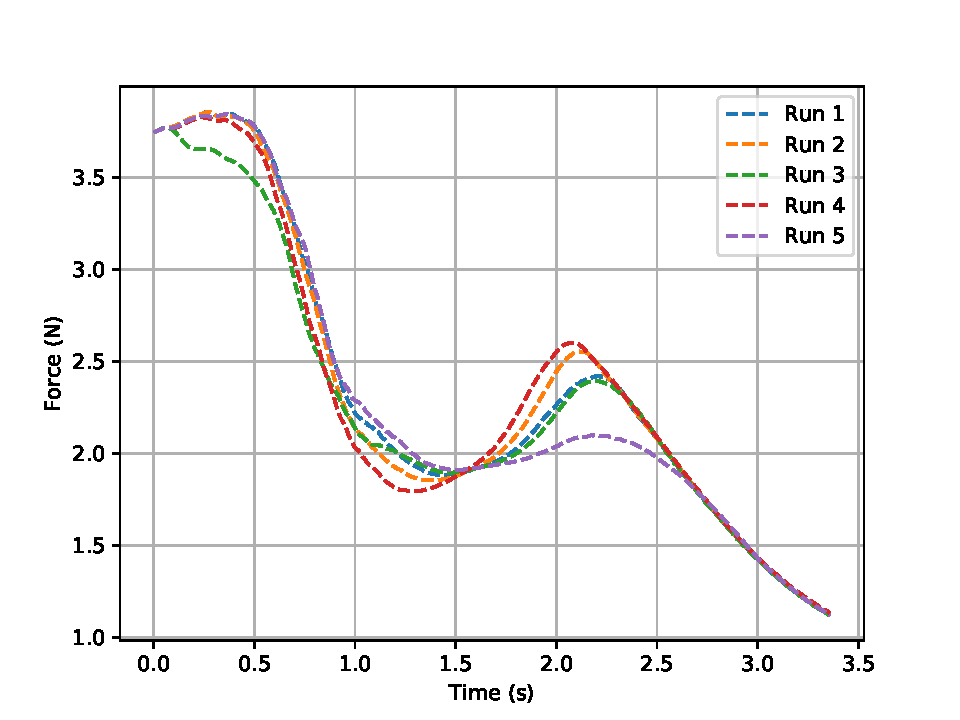
\includegraphics[width=\textwidth]{images/exp/cut/power_f2}
			\caption{\scriptsize Force generated by Gaussian policy while cutting vegetable}
		\end{figure}
	\end{minipage}
	\hfill
	\begin{minipage}[t]{0.49\textwidth}
		
		\begin{figure}
			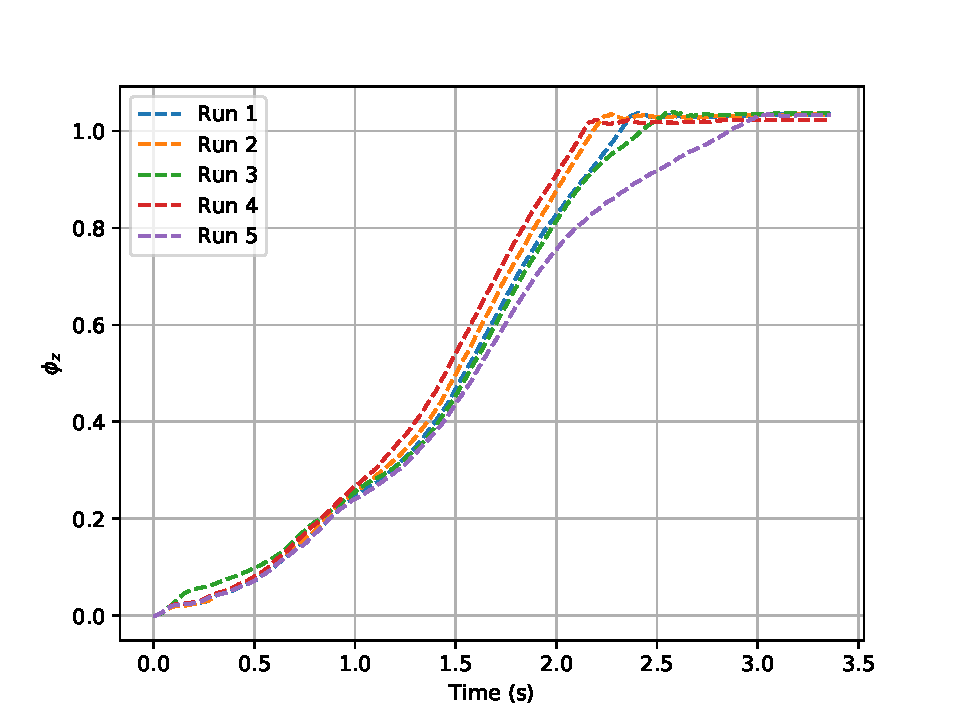
\includegraphics[width=\textwidth]{images/exp/cut/power_ph_z2}
			\caption{\scriptsize Cutting phase $\phi_{z}$ in Z-direction}
		\end{figure}
	\end{minipage}
\end{frame}


\begin{frame}
	Learning Force Policy with PoWER Algorithm
	\vspace{-0.3cm}
	\scriptsize
	\begin{figure*}[t]
		\begin{subfigure}[t]{0.32\textwidth}
			\centering
			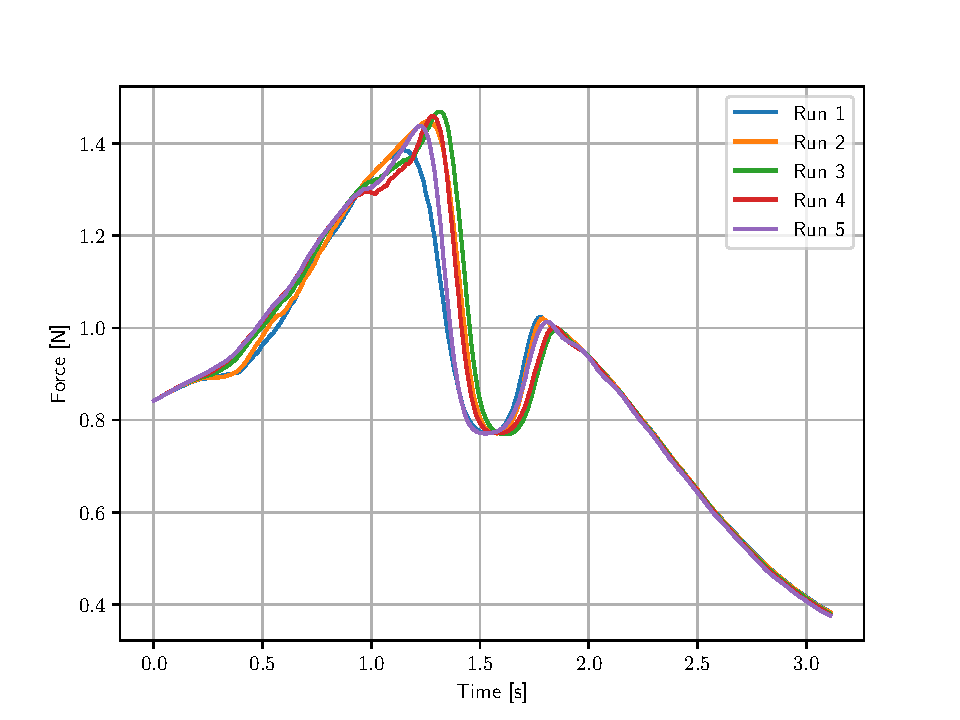
\includegraphics[width=\textwidth]{images/f_banana_1.pdf}
					\vspace{-0.32cm}
			\caption{\scriptsize 1 day old}
			\label{EX:f_banana_1}
		\end{subfigure}
		\begin{subfigure}[t]{0.32\textwidth}
			\centering
			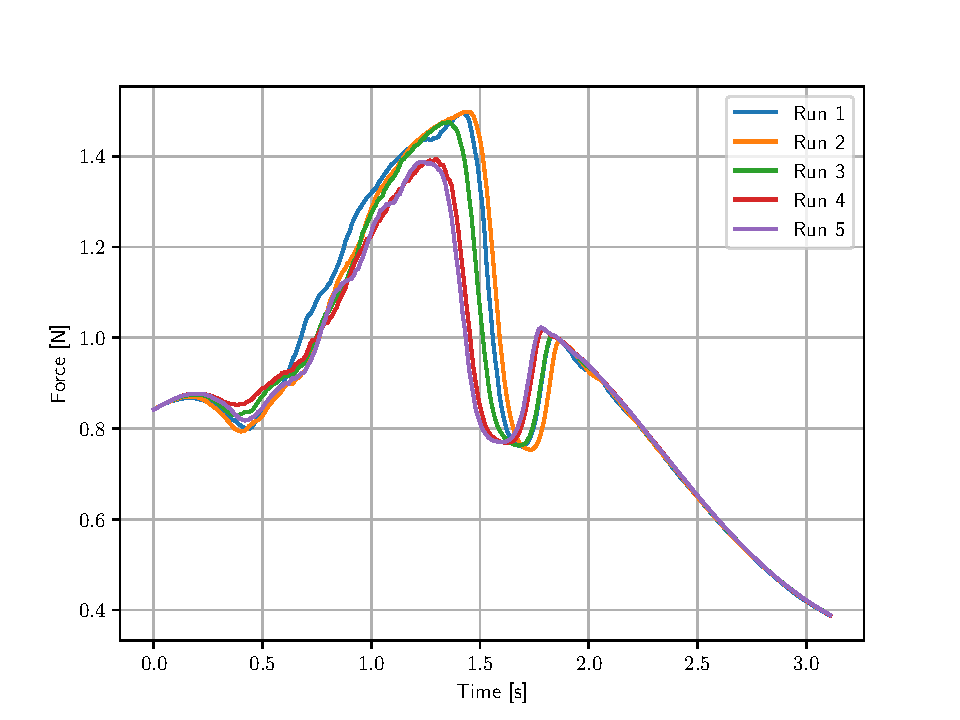
\includegraphics[width=\textwidth]{images/f_banana_2.pdf}
					\vspace{-0.32cm}
			\caption{\scriptsize 2 days old}
			\label{EX:f_banana_2}
		\end{subfigure}
		\begin{subfigure}[t]{0.32\textwidth}
			\centering
			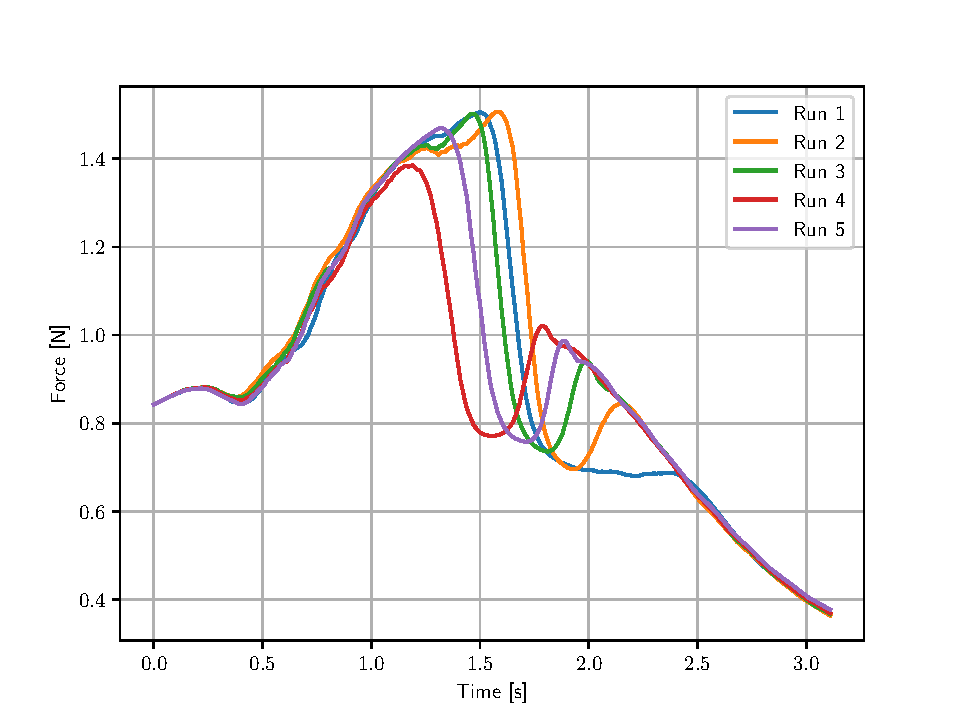
\includegraphics[width=\textwidth]{images/f_banana_3.pdf}
			\vspace{-0.32cm}
			\caption{\scriptsize 3 days old}
			\label{EX:f_banana_3}
		\end{subfigure}
		\vspace{-0.5cm}
		\caption{Force applied at TCP in $Z$-direction for cutting bananas with different ripeness.}
		\label{EX:f_banana}
	\end{figure*}
	\vspace{-0.85cm}
\begin{figure*}[t]
	\begin{subfigure}[t]{0.32\linewidth}
		\centering
		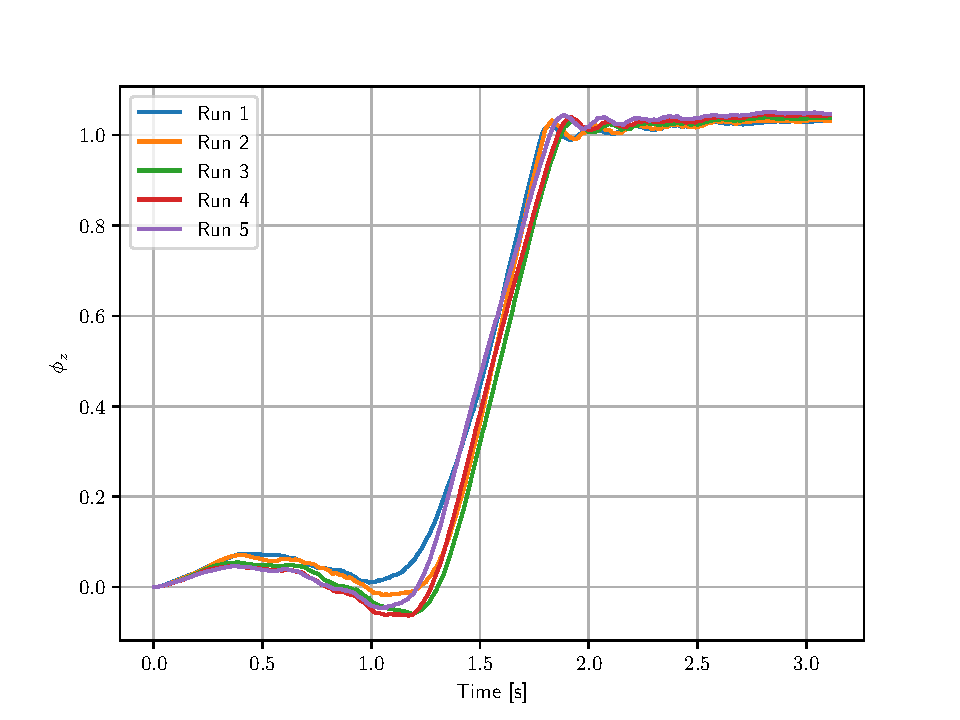
\includegraphics[width=\textwidth]{images/ph_banana_1.pdf}
\vspace{-0.32cm}
\caption{\scriptsize 1 days old}
		\label{EX:ph_banana_1}
	\end{subfigure}
	\begin{subfigure}[t]{0.32\linewidth}
		\centering
		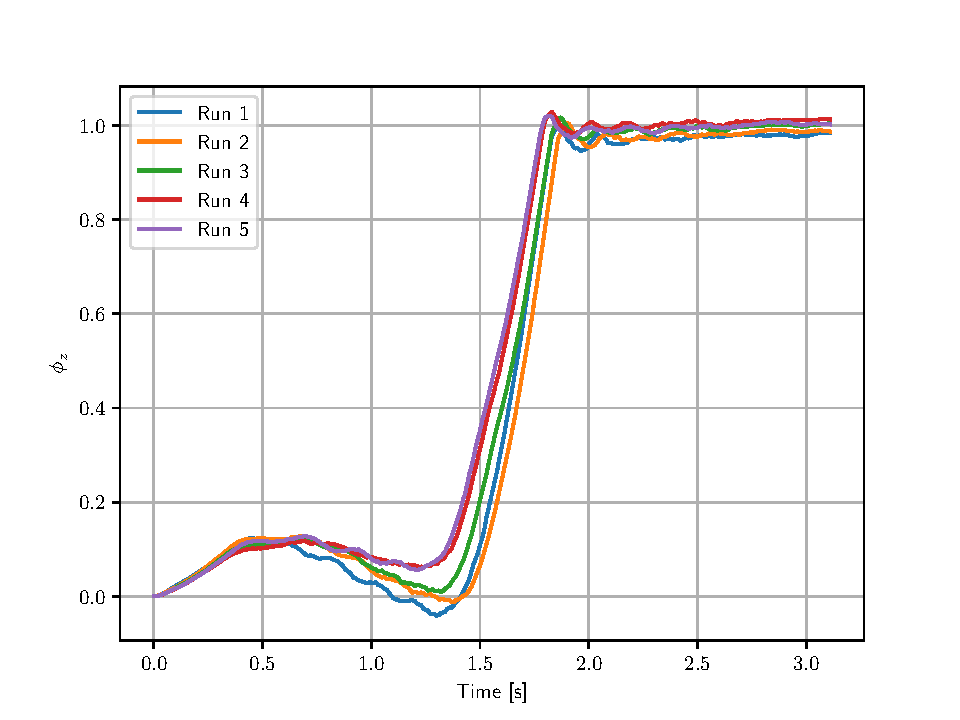
\includegraphics[width=\textwidth]{images/ph_banana_2.pdf}
\vspace{-0.32cm}
\caption{\scriptsize 2 days old}
		\label{EX:ph_banana_2}
	\end{subfigure}
	\begin{subfigure}[t]{0.32\linewidth}
		\centering
		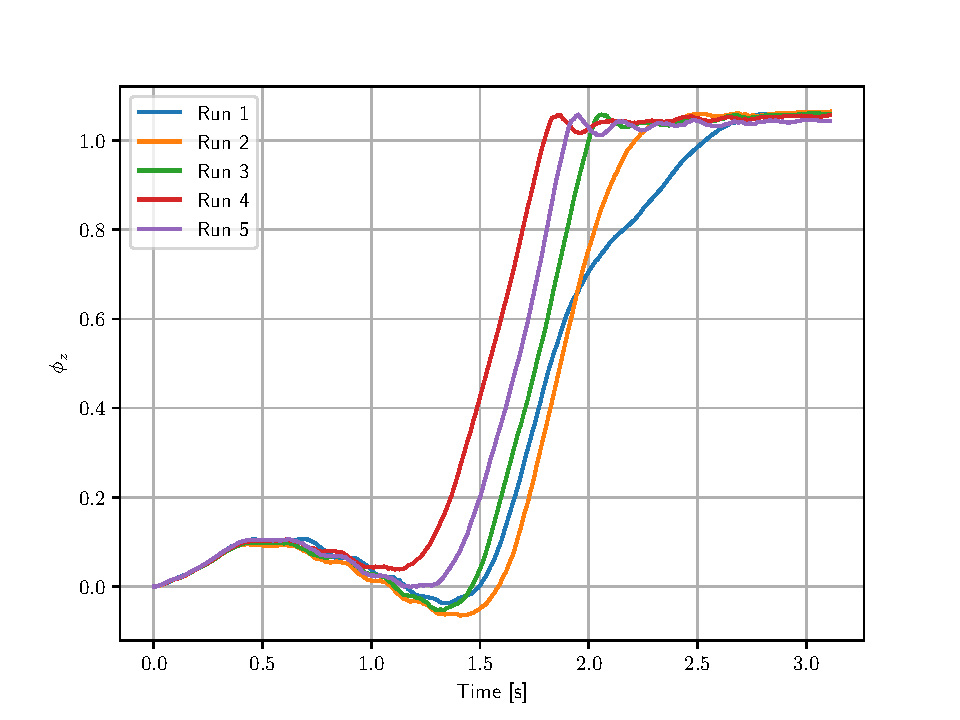
\includegraphics[width=\textwidth]{images/ph_banana_3.pdf}
\vspace{-0.32cm}
\caption{\scriptsize 3 days old}
		\label{EX:ph_banana_3}
	\end{subfigure}
	\vspace{-0.5cm}
	\caption{Phase $\phi_z$ of the cutting motion in $Z$-direction for cutting bananas with different ripeness.}
	\label{EX:ph_banana}
\end{figure*}
\end{frame}


\begin{frame}{Discussion}
	\begin{itemize}
		\item REINFORCE algorithm failed to learn force policy for cutting vegetables because of ineffective exploration with high frequency noise in low-pass filter like environment.
		\item Increase in policy parameters resulted in increase in number of trials required for learning.
		\item It was also observed that the cutting depth achieved in previous trial affected the return of the next trial due to more resistance provided by vegetable.
		\item Different noise variance should be used for different parameters.
	\end{itemize}
\end{frame}




\begin{frame}{Conclusions}
	\vspace{-1cm}	

	\newgeometry{textwidth=14.53cm}
	\begin{minipage}[t]{0.49\textwidth}
		\begin{itemize}
			\small
			\item Generalization ability of door opening approach - tested on two different robots.
			\item Extension for detecting the opening direction of the door and if the door is jammed.
			\item Oscillations in the end-effector trajectory while opening door due to sensor noise and low command update rate.		
			\item Force policies for cutting vegetable were learned using PoWER algorithm with linear and Gaussian policy representation.
		\end{itemize}
	\end{minipage}
	\hfill
	\begin{minipage}[t]{0.49\textwidth}
		\begin{itemize}
			\small
	
			\item Task specification framework reduced the dimensions of the problem from six to one, which resulted in faster learning directly on the robot without using simulation.
			\item Simple policies can be very effective when one is interested in learning to perform the task rather than learning the complex dynamics of the environment in which the task is being performed.
			\item The choice of the reinforcement learning algorithm is affected by the task dynamics.
			
		\end{itemize}
	\end{minipage}
\end{frame}

\begin{frame}{Future Work}
	%\vskip1ex
	\begin{minipage}[t]{0.51\textwidth}
		\begin{itemize}
			\small  
			\item Auto-tuning methods for tuning of admittance controller parameters.
			\item Extending the approach for tasks such as sweeping the floor, cutting curtains and bags during an investigation of the potentially dangerous environment.
		
		\end{itemize}
	\end{minipage}
	\hfill
	\begin{minipage}[t]{0.47\textwidth}
		\begin{itemize}
			\small 
			\item Extending  for tasks involving multi-directional force interactions with the environment such as collaborating with human to transport objects from one place to another.
		\end{itemize}
	\end{minipage}
\end{frame}

\begin{frame}[allowframebreaks]{References}
	
	\bibliography{../../project-proposal/bibliography}
	\bibliographystyle{abbrv}
	
\end{frame}


\end{document}
